% last update november 2019
\documentclass{esannV2}
\usepackage[dvips]{graphicx}
\usepackage[utf8]{inputenc}
\usepackage{amssymb,amsmath,array}
\usepackage{hyperref}
\usepackage{booktabs}
\usepackage{tikz}
\usetikzlibrary{positioning,shapes.geometric,arrows.meta,calc}

%***********************************************************************
% !!!! IMPORTANT NOTICE ON TEXT MARGINS !!!!!
%***********************************************************************
%
% Please avoid using DVI2PDF or PS2PDF converters: some undesired
% shifting/scaling may occur when using these programs
% It is strongly recommended to use the DVIPS converters, and to submit
% PS file. You may submit a PDF file if and only if you use ADOBE ACROBAT
% to convert your PS file to PDF.
%
% Check that you have set the paper size to A4 (and NOT to letter) in your
% dvi2ps converter, in Adobe Acrobat if you use it, and in any printer driver
% that you could use.  You also have to disable the 'scale to fit paper' option
% of your printer driver.
%
% In any case, please check carefully that the final size of the top and
% bottom margins is 5.2 cm and of the left and right margins is 4.4 cm.
% It is your responsibility to verify this important requirement.  If these margin requirements and not fulfilled at the end of your file generation process, please use the following commands to correct them.  Otherwise, please do not modify these commands.
%
\voffset 0 cm \hoffset 0 cm \addtolength{\textwidth}{0cm}
\addtolength{\textheight}{0cm}\addtolength{\leftmargin}{0cm}

%***********************************************************************
% !!!! USE OF THE esannV2 LaTeX STYLE FILE !!!!!
%***********************************************************************
%
% Some commands are inserted in the following .tex example file.  Therefore to
% set up your ESANN submission, please use this file and modify it to insert
% your text, rather than staring from a blank .tex file.  In this way, you will
% have the commands inserted in the right place.

\begin{document}
%style file for ESANN manuscripts
\title{See Without Decoding: Motion-Vector-Based Tracking in Compressed Video}

%***********************************************************************
% AUTHORS INFORMATION AREA
%***********************************************************************
\author{Duch\'e Axel$^{1,2}$, Gasso Gilles$^2$ and Chatelain Cl\'ement $^2$
%
% Optional short acknowledgment: remove next line if non-needed
\thanks{This work was supported by the ANRT under a CIFRE contract with Actemium Paris Transport.}
%
% DO NOT MODIFY THE FOLLOWING '\vspace' ARGUMENT
\vspace{.3cm}\\
%
% Addresses and institutions (remove "1- " in case of a single institution)
1- Actemium Paris Transport, %\\
%24 Bd de Pesaro, 92000 
Nanterre - France\\
%
% Remove the next three lines in case of a single institution
2- INSA Rouen, LITIS UR 4108, Saint-Étienne-du-Rouvray - France
}
%***********************************************************************
% END OF AUTHORS INFORMATION AREA
%***********************************************************************

\maketitle

\begin{abstract}
We propose a lightweight \textbf{compressed-domain tracking model} that operates directly on video streams, eliminating the need for full RGB decompression and storage. Using motion vectors and transform coefficients extracted from compressed data, our method efficiently propagates object bounding boxes across frames, reducing computational cost by up to $7\times$ with only a 4\% drop in mAP@0.5 compared to an RGB baseline on the MOTS15, MOTS17, and MOTS20 benchmarks. These results highlight the efficiency and scalability of codec-domain motion modeling for real-time analytics in large monitoring systems.
\end{abstract}

\section{Introduction}
\label{sec:intro}

Modern cities operate extensive camera networks across transportation hubs, public areas, and sensitive zones. These systems must deliver reliable, continuous analytics---including motion detection, intrusion monitoring, and behavior analysis---under strict constraints on computation, storage, and energy consumption across thousands of concurrent video streams. Conventional image-domain preprocessing~\cite{PIDS_Survey_2022} (e.g., background subtraction or frame differencing) offers low-cost activity filtering but remains fragile under illumination changes, vibrations and clutter.

Deep learning--based vision models have substantially improved robustness and precision while maintaining a good balance between speed and accuracy, as seen in recent architectures such as RT-DETR~\cite{detrs_beat_yolos_2024} and the latest YOLO versions~\cite{khanam2024yolov11overviewkeyarchitectural}. However, most vision pipelines still rely on fully decoded RGB frames, which are computationally heavy and memory-intensive to process. Performing real-time inference on high-resolution RGB data requires powerful GPUs or specialized hardware, making large-scale deployment difficult and energy-intensive. This dependency on heavy RGB processing represents a fundamental scalability barrier for camera networks.

We address this limitation by starting from a simple hypothesis: compressed video streams already carry most of the spatial–temporal information required for tracking. In particular, motion vectors and transform coefficients estimated by the codec can be reused as meaningful motion and appearance cues without explicit RGB reconstruction. Building on this assumption, we propose a lightweight hybrid architecture that performs a single detection on an initial decoded RGB frame, followed by tracking and refinement of bounding boxes directly from codec-domain features. By leveraging information already available in the stream, the system avoids redundant pixel-level computation while maintaining competitive accuracy, supporting scalable and energy-efficient analytics across large camera infrastructures.


Hereafter, we briefly review prior research on compressed-domain video understanding and how existing strategies balance efficiency and accuracy under similar constraints.


\section{Related Work and Positioning}
\label{sec:sota}

Video understanding from compressed data aims to perform tasks such as \emph{object detection, tracking, and classification} directly from encoded video streams without unnecessary reconstruction.  
This setting is increasingly relevant for large-scale surveillance and analytics systems, where thousands of compressed feeds must be processed under strict computational and energy constraints.  
Existing research can be broadly categorized by the degree of \emph{decompression} used during inference: full, partial, or none.

\paragraph{Full decoding.}
Conventional pipelines fully reconstruct RGB frames before analysis.  
They rely on convolutional or transformer-based models to detect and track objects in the pixel domain, achieving high accuracy but at considerable computational cost.  
Even motion-assisted variants such as MV-YOLO~\cite{mv_yolo_motion_vector_2018} integrate motion cues only after full decoding, offering limited gains in scalability or efficiency.

\paragraph{Partial decoding.}
To reduce overhead, some studies leverage motion and residual information computed by the codec while still decoding part of the image.  
Frame-group aggregation methods~\cite{wang2019fastobjectdetectioncompressed,Wang_2021} process short sequences of partially decoded frames to exploit temporal redundancy, improving stability but adding aggregation components that hinder real-time operation.  
Other hybrid designs~\cite{Fast_Object_Detection_in_High-Resolution_Videos_2023} decode small regions or key patches while combining them with motion cues from the bitstream.  
However, because video data are sequentially encoded, even partial decoding typically requires decompressing earlier segments, which limits the achievable efficiency.

\paragraph{No-decoding methods.}
Recent work investigates learning directly from compressed signals without reconstructing RGB pixels.  
Our previous studies~\cite{dct_detection_2019,dct_luminance_2021} showed that frequency-domain features preserve sufficient structure for spatial localization tasks.  
Building on this idea, we propose a lightweight \emph{tracking model} that performs a single detection on an initial decoded frame and then updates bounding boxes using only motion vectors and transform coefficients from the compressed stream.  
Unlike fully or partially decoded approaches, our formulation removes the need for repeated RGB reconstruction and heavy temporal aggregation, operating entirely on data already present in the bitstream.  
This design retains essential motion and appearance cues while drastically lowering computational cost, making it suitable for real-time, large-scale video analytics.


\section{Compressed Video Representation and Feature Extraction}
\label{sec:compressed_representation}

Our objective is to transform a compressed video stream into a compact tensor representation suitable for tracking and detection.  
The \textbf{input} is an MPEG-4 encoded stream, and the \textbf{output} consists of two feature maps per frame: a motion field and a transform-energy map derived from the encoder’s internal data.  
This allows the model to reason on motion and appearance cues without reconstructing RGB images.

\paragraph{Encoded features.}
During compression, the video encoder estimates how image regions move and how their appearance changes.  
Two main signals are produced:
\begin{itemize}
    \item \textbf{Motion vectors (MV):} 2D displacement fields describing how $16\times16$ pixel blocks move between consecutive frames, similar to a coarse optical flow estimated by the codec.
    \item \textbf{Discrete Cosine Transform (DCT) coefficients:} frequency-domain components capturing residual appearance differences—edges, textures, and local luminance changes.
\end{itemize}
These quantities are computed automatically by the encoder and can be extracted directly from the bitstream at minimal cost.

\paragraph{Compressed sequence structure.}
A video is organized as a series of \emph{Groups of Pictures} (GOPs), denoted $\mathcal{G}^g=\{f_0^g, f_1^g, \ldots, f_N^g\}$, where $g$ indexes the GOP, $N$ its number of frames, and $f_n^g$ the $n$-th frame within it.  
The first frame $f_0^g$ is an intra-coded (\textbf{I}) frame that stores a full image, while the following frames $f_n^g$ ($n>0$) are predictive (\textbf{P}) frames that reference earlier images through motion vectors and DCT-encoded residuals.  
Each predictive frame can therefore be represented as:
\[
f_n^g = \{MV_n^g, \mathcal{DCT}(\Delta Y_n^g)\},
\qquad
f_0^g = \{\mathcal{DCT}(Y_0^g)\},
\]
where $\Delta Y_n^g$ denotes the luminance residual (difference from the reference frame).  
This structure yields a compact yet information-rich description of motion and texture (Table~\ref{tab:data_ratio}).

\begin{table}[h]
\centering
\setlength{\tabcolsep}{6pt}
\renewcommand{\arraystretch}{1.0}
\caption{Relative data size per frame (640$\times$640 input, RGB baseline = 1.0$\times$).}
\label{tab:data_ratio}
\begin{tabular}{|l|c|c|}
\hline
\textbf{Representation} & \textbf{Resolution} & \textbf{Size Ratio} \\
\hline
Motion vectors & 40$\times$40 & 0.012$\times$ \\
DCT residuals (Y) & 80$\times$80 & 0.16$\times$ \\
\hline
\end{tabular}
\end{table}


\paragraph{Partial decompression.}
We directly parse motion vectors and low-frequency DCT coefficients from the bitstream, omitting inverse transforms and color conversion.  
This preserves spatial–temporal cues while cutting decoding time by over threefold.  
Our open-source extractor\footnote{\url{https://github.com/your-repo-name}} outputs MV and DCT tensors for learning (Fig.~\ref{fig:compression_pipeline}).

\begin{figure}[h!]
\centering
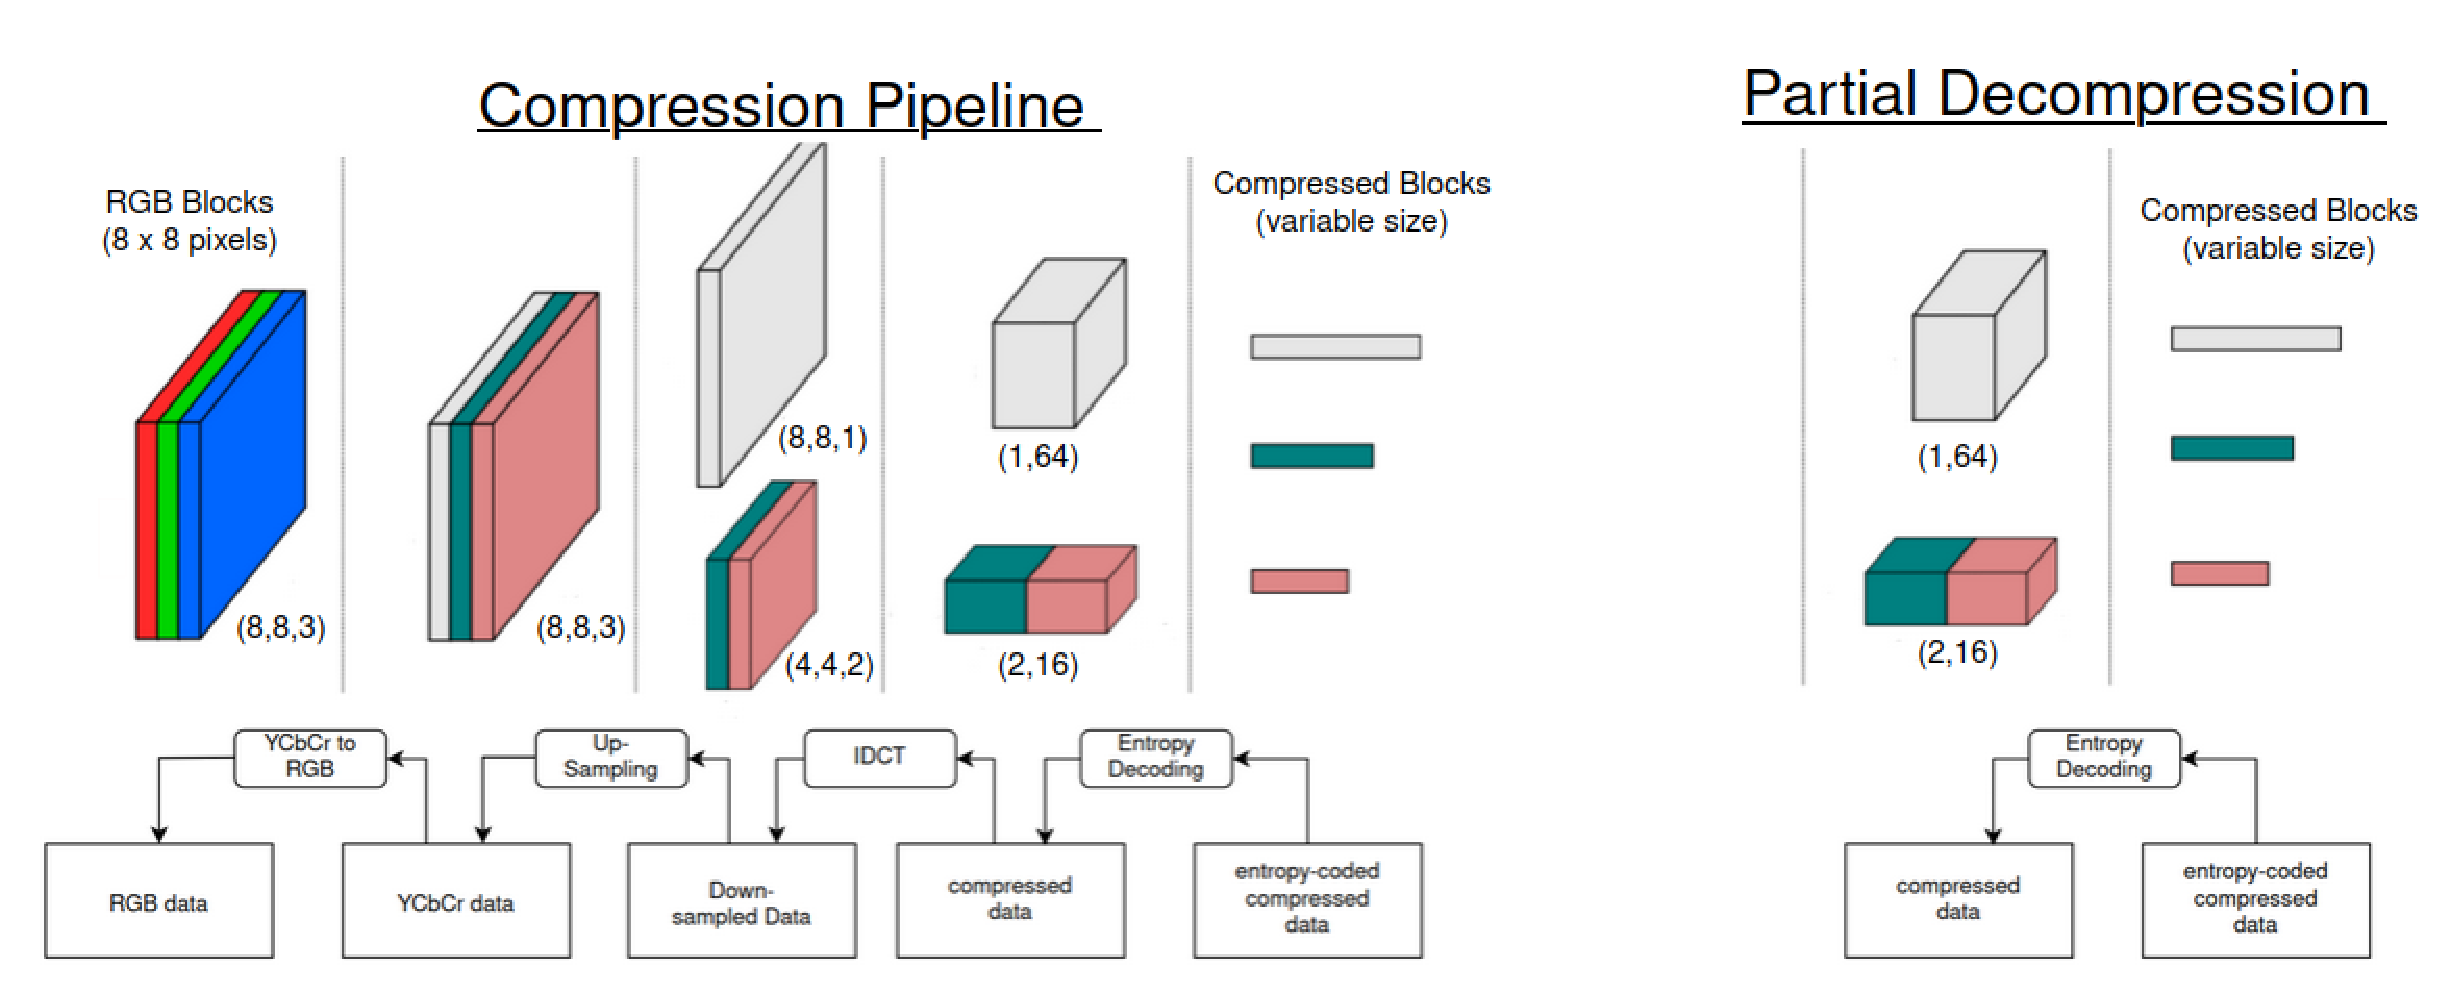
\includegraphics[width=0.90\linewidth]{figs/compression_pipeline.eps}
\caption{Standard MPEG-4 decoding (left) vs.\ our partial pipeline (right), which outputs motion and DCT tensors directly.}
\label{fig:compression_pipeline}
\vspace{-0.6em}
\end{figure}

\paragraph{Efficiency.}
The extractor achieves a \textbf{3--4$\times$} speed-up versus full RGB decoding (Table~\ref{tab:speed_decompression}) while retaining motion and frequency cues required for accurate propagation.

\begin{table}[h]
\centering
\setlength{\tabcolsep}{6pt}
\renewcommand{\arraystretch}{1.0}
\caption{Average decoding time on MOTS datasets (lower is better).}
\label{tab:speed_decompression}
\begin{tabular}{|l|c|c|c|}
\hline
Metric & RGB & Partial SOTA & \textbf{Ours} \\
\hline
ms / P-frame & 6.67 & 2.48 ($\times0.37$) & \textbf{2.22 ($\times0.33$)} \\
ms / I-frame & 8.62 & 4.29 ($\times0.50$) & \textbf{2.50 ($\times0.29$)} \\
ms / GOP     & 83.33 & 32.26 ($\times0.39$) & \textbf{27.03 ($\times0.32$)} \\
\hline
\end{tabular}
\end{table}

\noindent\textbf{Summary.}
MPEG-4 motion and transform data provide dense motion and structure cues at a fraction of the size of RGB frames, forming an efficient interface for our propagation model described next.




\noindent\textbf{Summary.}
MPEG-4 motion and transform data provide dense motion and structure cues at a fraction of the size of RGB frames, forming an efficient interface for our propagation model described next.

\section{Lightweight Propagation Architecture}
\label{sec:architecture}

Our approach performs a single detection on the decoded I-frame $f_0^g$, then propagates bounding boxes across P-frames using only codec features. We propose two architectural variants: a \textbf{Fast} global-pooling design for real-time operation, and an \textbf{ROI-based} variant that extracts box-aligned features for improved accuracy. Figure~\ref{fig:roi_architecture} illustrates the ROI-based approach.

\begin{figure}[t!]
\centering
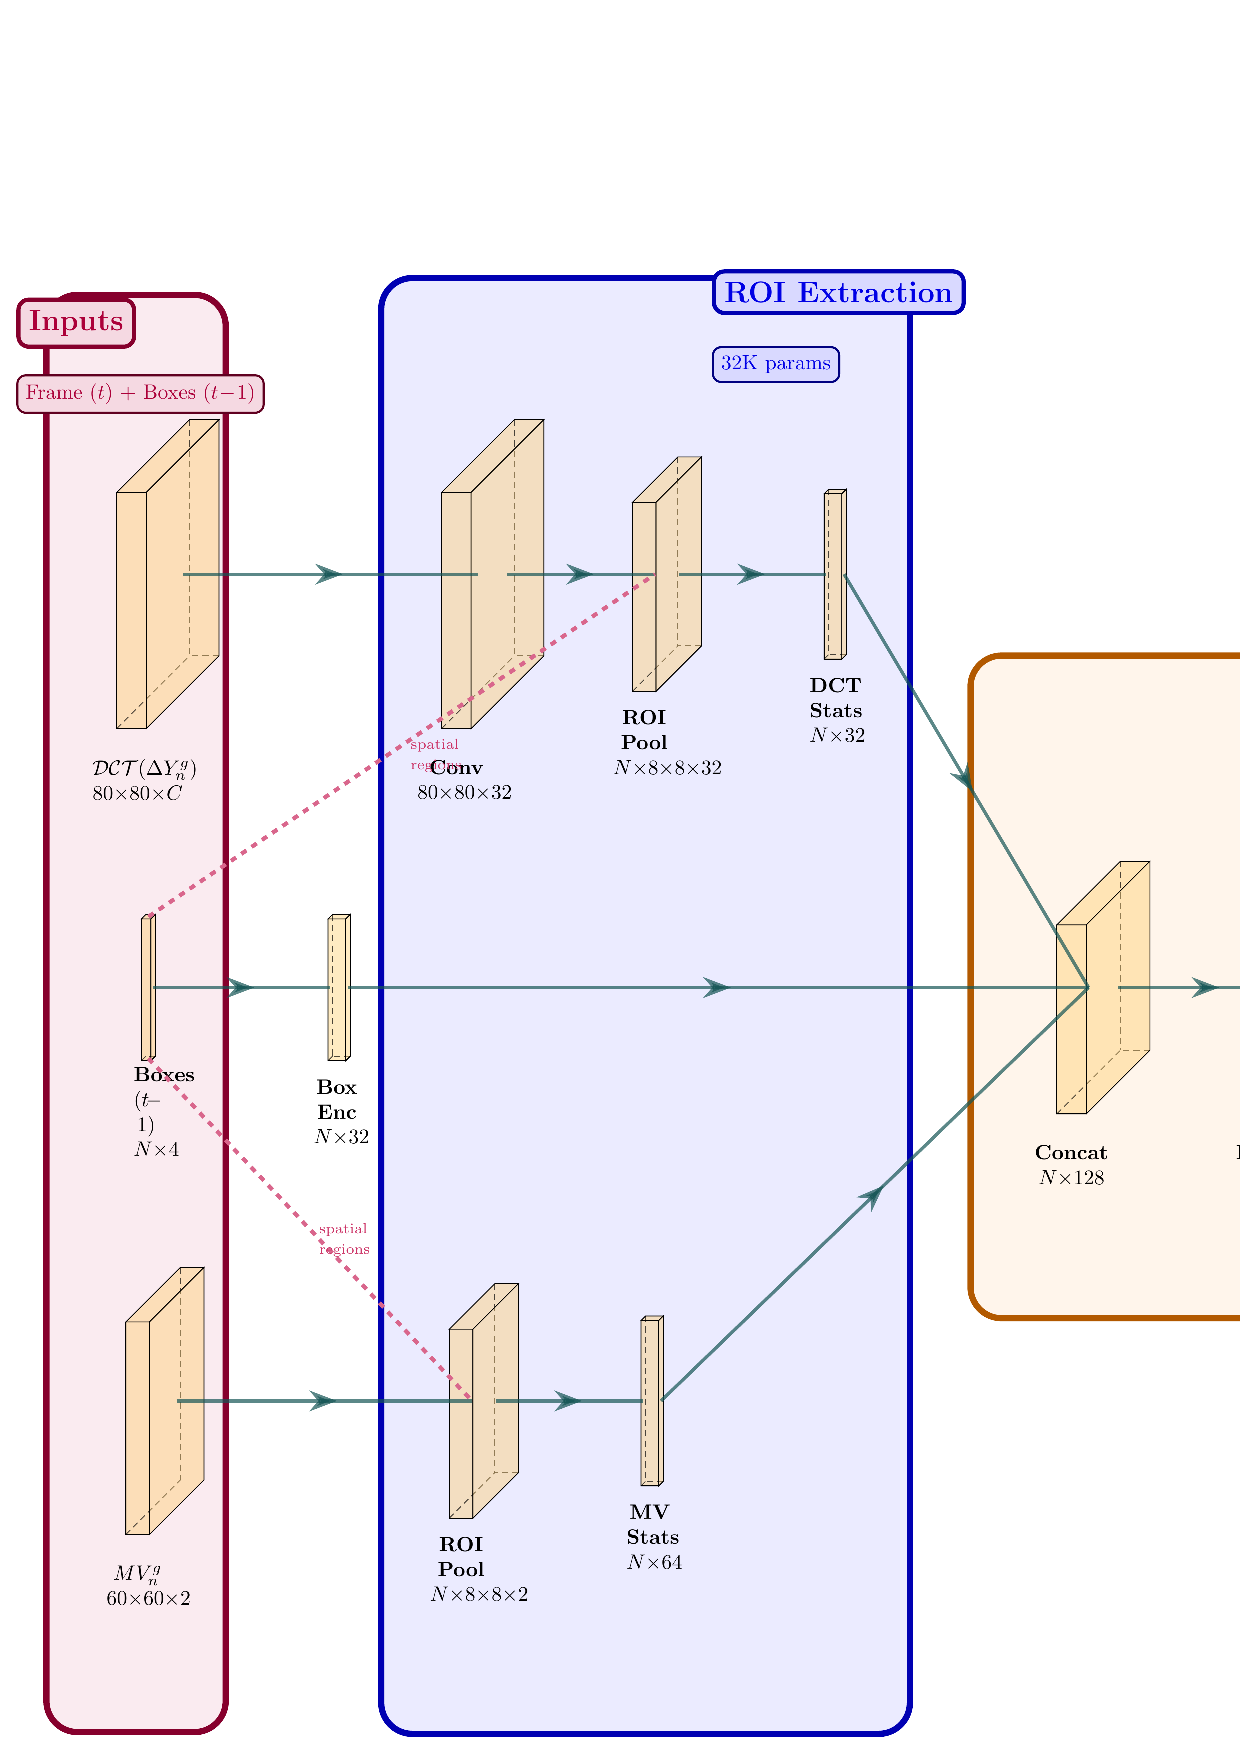
\includegraphics[width=0.98\linewidth]{figs/roi_architecture.png}
\caption{ROI-based propagation architecture. Bounding boxes from frame $(t\!-\!1)$ define spatial regions (dashed lines) for extracting box-aligned features from $MV_n^g$ (60$\times$60$\times$2) and $\mathcal{DCT}(\Delta Y_n^g)$ (80$\times$80$\times$C). ROI pooling produces fixed-size 8$\times$8 feature maps per box, which are processed into per-box statistics (N$\times$64 for MV, N$\times$32 for DCT) and fused with box encodings (N$\times$32). A BiLSTM integrates temporal context before prediction heads output updated boxes at frame $t$. Total: $\sim$230K params.}
\label{fig:roi_architecture}
\vspace{-0.8em}
\end{figure}

\paragraph{ROI Extraction (32K params).}
Given $N$ bounding boxes from frame $(t\!-\!1)$, we extract box-aligned features from motion and DCT maps:
\begin{itemize}
\item \textbf{MV branch}: $MV_n^g \in \mathbb{R}^{60 \times 60 \times 2}$ undergoes ROI pooling to produce $N\times8\times8\times2$ features, then statistics (mean, std, range) yield $N\times64$ per-box descriptors.
\item \textbf{DCT branch}: $\mathcal{DCT}(\Delta Y_n^g) \in \mathbb{R}^{80 \times 80 \times C}$ passes through 3$\times$3 convolution (32 channels), ROI pooling ($N\times8\times8\times32$), and statistics to obtain $N\times32$ descriptors.
\item \textbf{Box encoding}: Normalized coordinates $(c_x, c_y, w, h)$ are embedded to $N\times32$ via a small MLP.
\end{itemize}

\paragraph{Fusion \& Temporal (196K params).}
Per-box features (64 MV + 32 DCT + 32 box = 128 dims) are concatenated, yielding $N\times128$ inputs. A BiLSTM (128 hidden units) processes the sequence, modeling temporal dependencies across the GOP. Finally, two prediction heads output position deltas ($\Delta$pos, $N\times2$) and size deltas ($\Delta$size, $N\times2$), which update the boxes for frame $t$.

\paragraph{Training.}
We train end-to-end on 200 GOPs from MOT15/17/20 (50 frames/GOP, 960$\times$960 resolution) using DETR-style detection loss with Hungarian matching: focal loss ($\alpha$=0.25, $\gamma$=2.0, weight=2.0), L1 regression (weight=5.0), and GIoU loss (weight=2.0).

\section{Experimental Results}
\label{sec:results}

\paragraph{Datasets \& Baselines.}
We evaluate on MOT15 (11 sequences), MOT17 (7 sequences), and MOT20 (4 sequences) across static (97 GOPs) and moving cameras (94 GOPs). Baselines: (1)~\textbf{Static I-frame} — propagate $f_0^g$ detections unchanged across all frames (ideal for static objects); (2)~\textbf{Mean MV} — apply per-frame average motion vector per box, updating positions autoregressively (expected to work on static cameras but fail on moving cameras due to camera motion contamination).

\paragraph{Theoretical Expectations.}
\textit{Static I-frame} should perform well on static cameras where objects move slowly relative to GOP length (50 frames), degrading as object displacement increases. It should maintain constant performance on moving cameras since it ignores motion entirely.
\textit{Mean MV} should provide moderate improvement over static propagation when objects move consistently on static cameras, but catastrophically fail on moving cameras where camera motion dominates object motion, making averaged vectors unreliable for box updates.
Our \textit{ROI model} should substantially outperform both baselines by learning per-box motion patterns, handling complex trajectories, and remaining robust to camera motion through learned codec features.

\paragraph{Results.}
Table~\ref{tab:results_compact} shows mAP@0.5 comparing our ROI-based model with baselines. On \textbf{static cameras}, learned propagation achieves \textbf{0.6856 mAP} (GOP-weighted average), approaching the Static I-frame baseline (0.6494, -5.6\%) while substantially outperforming Mean MV (0.4306, +59.2\%). 

Notably, performance varies significantly across datasets based on object motion characteristics. On \textbf{MOT15}, our model (0.6373 per-dataset) \textit{exceeds} the static baseline (0.5034) by \textbf{26.6\%}---the largest improvement across all datasets. This substantial gain occurs because MOT15 sequences exhibit the most significant object displacement relative to GOP length (50 frames): pedestrians frequently traverse the entire frame within a single GOP, making static box propagation increasingly inaccurate over time. Our learned temporal model compensates for this cumulative drift by integrating motion vectors and appearance cues through BiLSTM, successfully tracking objects across large displacements. Conversely, on \textbf{MOT17} (0.8050 vs. 0.8287 I-frame, -2.9\%) and \textbf{MOT20} (0.6747 vs. 0.7030, -4.0\%), objects move more slowly relative to frame rate, allowing static propagation to maintain high accuracy while reducing the relative benefit of learned motion modeling.

\begin{table}[h!]
\centering
\setlength{\tabcolsep}{3.0pt}
\renewcommand{\arraystretch}{1.05}
\caption{ROI-based model performance on static cameras (GOP-50, mAP@0.5).}
\label{tab:results_compact}
\begin{tabular}{|l|c|ccc|}
\hline
\textbf{Dataset} & \textbf{GOPs} & \textbf{Static I-frame} & \textbf{Mean MV} & \textbf{ROI Model} \\
\hline
MOT17 & 19 & 0.8287 & 0.6880 & \textbf{0.8050} \\
MOT15 & 38 & 0.5034 & 0.3079 & \textbf{0.6373} \\
MOT20 & 40 & 0.7030 & 0.4250 & 0.6747 \\
\hline
\textbf{Weighted Average} & \textbf{97} & \textbf{0.6494} & \textbf{0.4306} & \textbf{0.6856} \\
\hline
\end{tabular}
\vspace{-0.5em}
\end{table}

On \textbf{moving cameras}, our model achieves \textbf{0.3945 mAP}, dramatically outperforming Mean MV (0.0790, +399\%) which fails catastrophically as predicted, and closely matching the Static I-frame baseline (0.4154, -5.0\%). This near-parity is significant: it confirms our model learns camera-invariant object tracking, whereas naive motion averaging collapses when camera motion dominates (MOT17: +1410\% improvement over Mean MV). The slight gap suggests room for explicit camera motion compensation in future work.

\paragraph{Short GOP Performance.}
To assess accuracy under minimal propagation error (short temporal horizons), we evaluate on 6-frame GOPs where objects move minimally between I-frames. Table~\ref{tab:ablation_6p} compares compressed-domain variants against an RGB baseline (RT-DETR on every frame). All variants achieve competitive performance within 4--9\% of full RGB decoding, with MV-only achieving the best trade-off (0.8077 mAP, -4.0\%). This validates that codec features retain sufficient information for accurate localization even when appearance dominates over motion, demonstrating the approach's versatility across different GOP configurations.

\begin{table}[h!]
\centering
\setlength{\tabcolsep}{4pt}
\renewcommand{\arraystretch}{1.05}
\caption{Short GOP (6P) mAP@0.5: Compressed Domain vs RGB Baseline (Static Cameras)}
\label{tab:ablation_6p}
\begin{tabular}{lcccc}
\toprule
\textbf{Variant} & \textbf{Val mAP} & \textbf{Static (6P)} & \textbf{$\Delta$ vs RGB} & \textbf{$\Delta$ (\%)} \\
\midrule
RGB Baseline & --- & 0.8412 & --- & --- \\
\midrule
MV-only & 0.4922 & 0.8077 & -0.0335 & -4.0 \\
DCT-8 & 0.4884 & 0.7971 & -0.0441 & -5.2 \\
DCT-16 & 0.5019 & 0.8018 & -0.0394 & -4.7 \\
DCT-32 & 0.4778 & 0.7979 & -0.0433 & -5.2 \\
DCT-64 & 0.4761 & 0.8015 & -0.0397 & -4.7 \\
MV$+$DCT-8 & 0.4698 & 0.7986 & -0.0426 & -5.1 \\
MV$+$DCT-16 & 0.4743 & 0.7982 & -0.0430 & -5.1 \\
MV$+$DCT-32 & 0.5014 & 0.8015 & -0.0397 & -4.7 \\
MV$+$DCT-64 & 0.3495 & 0.7653 & -0.0759 & -9.0 \\
\bottomrule
\end{tabular}
\vspace{-0.5em}
\end{table}

\paragraph{Efficiency.}
The ROI-based architecture maintains computational efficiency through compact per-box features and shared parameters. Combining partial decompression (3--4$\times$ speedup, Table~\ref{tab:speed_decompression}) with lightweight architecture ($\sim$230K params vs. multi-million parameter RGB detectors), we achieve substantial speedup while enabling box-specific motion modeling. ROI pooling to fixed 8$\times$8 regions keeps memory footprint low even with many boxes (N=50: $\sim$200KB activations vs. $\sim$1MB for global pooling on full feature maps).

\paragraph{Deployment Scalability.}
Table~\ref{tab:speed_gop} demonstrates real-world deployment capacity on a single 16GB GPU. While RGB-based RT-DETR processes only \textbf{13 concurrent 30-FPS camera streams}, our compressed-domain approach scales dramatically: MV-only handles \textbf{301 streams} at GOP-50 (23$\times$ scaling), while even the heavier MV$+$DCT-64 variant supports \textbf{215 streams} (16.5$\times$ scaling). At shorter GOPs (GOP-6), throughput reaches 71 streams for lightweight variants. This scalability stems from: (1)~bypassing expensive RGB decoding for 98\% of frames (49/50 P-frames in GOP-50); (2)~compact codec features requiring minimal memory bandwidth; (3)~lightweight propagation networks. The results validate codec-domain tracking as a practical solution for large-scale surveillance networks where thousands of cameras must operate under strict computational budgets.

\begin{table}[h!]
\centering
\setlength{\tabcolsep}{4pt}
\renewcommand{\arraystretch}{1.05}
\caption{Deployment Capacity: RT-DETR (I-frame) + Compressed Domain (P-frames) on 16GB GPU}
\label{tab:speed_gop}
\begin{tabular}{lccc}
\toprule
\textbf{Variant} & \textbf{GOP-6} & \textbf{GOP-12} & \textbf{GOP-50} \\
 & \textbf{(1I+5P)} & \textbf{(1I+11P)} & \textbf{(1I+49P)} \\
 & \textbf{30 FPS} & \textbf{30 FPS} & \textbf{30 FPS} \\
\midrule
\textbf{RT-DETR (RGB)} & 13 & 13 & 13 \\
\midrule
MV-only & 71 & 126 & 301 \\
DCT-8 & 71 & 124 & 291 \\
DCT-16 & 71 & 125 & 292 \\
DCT-32 & 63 & 110 & 257 \\
DCT-64 & 55 & 98 & 232 \\
MV$+$DCT-8 & 69 & 118 & 256 \\
MV$+$DCT-16 & 69 & 119 & 263 \\
MV$+$DCT-32 & 61 & 106 & 231 \\
MV$+$DCT-64 & 54 & 95 & 215 \\
\bottomrule
\end{tabular}
\vspace{-0.5em}
\end{table}

\paragraph{Discussion.}
Our results demonstrate that codec-domain learned propagation achieves strong performance across diverse camera scenarios. On \textbf{static cameras}, the ROI model achieves 0.6856 mAP (GOP-weighted)---within 5.6\% of the Static I-frame baseline (0.6494) while dramatically outperforming naive Mean MV (+59.2\%). This confirms our hypothesis: learned box-aligned codec features enable robust tracking without requiring full decompression.

Three key findings emerge. First, the \textbf{MOT15 breakthrough} (0.6373 per-dataset vs. 0.5034 I-frame, +26.6\%) validates our core thesis that learned temporal modeling provides the greatest benefit when object motion is significant. MOT15 contains fast-moving pedestrians that traverse entire frames within 50-frame GOPs, causing static propagation to degrade rapidly as boxes drift from true positions. Our BiLSTM-based architecture learns to correct this accumulation error by fusing per-box motion statistics with appearance cues, maintaining accurate localization despite large displacements. In contrast, MOT17 and MOT20 feature slower object motion relative to temporal resolution, explaining why static propagation remains competitive (within 3--4\% of our model) and why the learned approach yields smaller gains. This performance pattern demonstrates that \textit{the value of temporal modeling scales with object displacement magnitude}---a critical insight for deployment: fast-motion scenarios (transportation hubs, sports venues) benefit most from our approach, while slow-motion settings may suffice with simpler baselines.

Second, the catastrophic failure of Mean MV on moving cameras (0.0790 mAP) confirms that camera motion contaminates averaged motion vectors---yet our model maintains 0.3945 mAP (+399\% improvement), demonstrating camera-invariant learning through encoded features. Third, the slight gap to Static I-frame on moving cameras (0.3945 vs. 0.4154, -5.0\%) suggests opportunity for explicit camera motion compensation in future work.

Architecturally, ROI pooling enables per-box feature extraction at scale (N=50 boxes: $\sim$200KB activations vs. $\sim$1MB for global pooling), while the compact 230K parameter model remains efficient compared to multi-million parameter RGB detectors. The results validate our core thesis: codec-domain tracking is \textit{viable} for real-world deployment when combining learned features, box-aligned representations, and temporal modeling. Future work will integrate appearance cues more deeply, explore camera motion compensation, and evaluate on longer GOP lengths to test autoregressive robustness.


% ****************************************************************************
% BIBLIOGRAPHY AREA
% ****************************************************************************

\begin{footnotesize}

% IF YOU DO NOT USE BIBTEX, USE THE FOLLOWING SAMPLE SCHEME FOR THE REFERENCES
% ----------------------------------------------------------------------------
\begin{thebibliography}{99}

% --- Core real-time detection & transformers ---

\bibitem{PIDS_Survey_2022}
D. Lohani, C. Crispim-Junior, Q. Barth\'elemy, S. Bertrand, L. Robinault and L. Tougne Rodet,
Perimeter Intrusion Detection by Video Surveillance: A Survey, MDPI, 2022

\bibitem{detrs_beat_yolos_2024}
Y. Zhao, W. Lv, S. Xu, J. Wei, G. Wang, Q. Dang, Y. Liu, and J. Chen,
``DETRs Beat YOLOs on Real-Time Object Detection, CVPR, 2024


\bibitem{khanam2024yolov11overviewkeyarchitectural}
R. Khanam and M. Hussain,
YOLOv11: An Overview of the Key Architectural Enhancements, ARXiV, 2024

\bibitem{mv_yolo_motion_vector_2018}
S. R. Alvar and I. V. Baji\'c,
MV-YOLO: Motion Vector-aided Tracking by Semantic Object Detection, IEEE International Workshop on Multimedia Signal Processing,  2018.

\bibitem{wang2019fastobjectdetectioncompressed}
S.~Wang, H.~Lu, and Z.~Deng, ``Fast Object Detection in Compressed Video, ICCV, 2018

\bibitem{Wang_2021}
X. Wang, Z. Huang, B. Liao, L. Huang, Y. Gong and C. Huang,
Real-time and accurate object detection in compressed video by long short-term feature aggregation, CVIU, May 2021.

\bibitem{Fast_Object_Detection_in_High-Resolution_Videos_2023}
R. Tran, A. Kanaujia and V. Parameswaran,
Fast Object Detection in High-Resolution Videos, ICCVW, October 2023.

\bibitem{dct_detection_2019}
B. Deguerre, C. Chatelain and G. Gasso,
Fast object detection in compressed JPEG images, ITSC , 2019.

\bibitem{dct_luminance_2021}
B. Deguerre, C. Chatelain and G. Gasso,
Object Detection in the DCT Domain: is Luminance the Solution, ICPR 2020

\bibitem{MOTS15}
L. Leal-Taix\'{e}, A. Milan, I. Reid, S. Roth, and K. Schindler,
``MOTChallenge 2015: Towards a Benchmark for Multi-Target Tracking

\bibitem{MOTS17}
A. Milan, L. Leal-Taix\'{e}, I. Reid, S. Roth, and K. Schindler,
``MOT16: A Benchmark for Multi-Object Tracking

\bibitem{MOTS20}
P. Dendorfer, H. Rezatofighi, A. Milan, J. Shi, D. Cremers, I. Reid, S. Roth, K. Schindler, and L. Leal-Taix\'{e},
``MOT20: A Benchmark for Multi-Object Tracking in Crowded Scenes
\end{thebibliography}

% ----------------------------------------------------------------------------

% IF YOU USE BIBTEX,
% - DELETE THE TEXT BETWEEN THE TWO ABOVE DASHED LINES
% - UNCOMMENT THE NEXT TWO LINES AND REPLACE 'Name_Of_Your_BibFile'

%\bibliographystyle{unsrt}
%\bibliography{Name_Of_Your_BibFile}

\end{footnotesize}

% ****************************************************************************
% END OF BIBLIOGRAPHY AREA
% ****************************************************************************

\end{document}
